\documentclass{standalone}
\usepackage{circuitikz}
\usepackage{amsmath}
\begin{document}
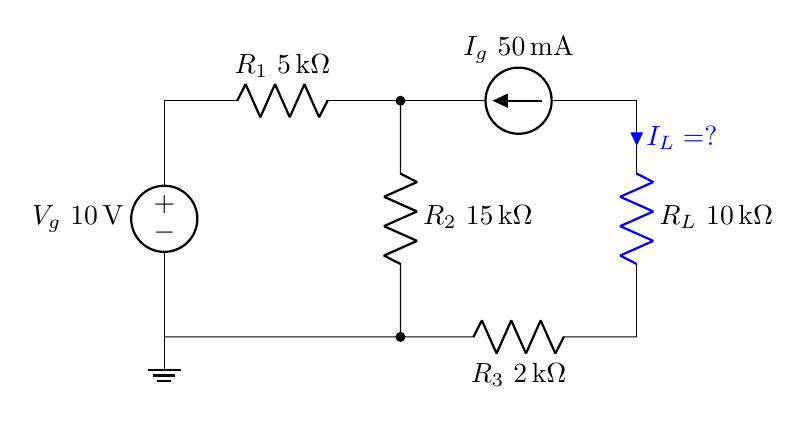
\begin{tikzpicture}[transform shape]
	% Paths, nodes and wires:
	\draw (-2, 2) to[american resistor, l={$R_1 \ 5\, \text{k}\Omega$}] (1, 2);
	\draw (1, 2) to[american resistor, l={$R_2 \ 15\, \text{k}\Omega$}] (1, -1);
	\draw (4, 2) to[american current source, mirror, l_={$I_g \ 50\, \text{mA}$}] (1, 2);
	\draw (1, -1) to[american resistor, l_={$R_3 \ 2\, \text{k}\Omega$}] (4, -1);
	\draw (-2, 2) to[american voltage source, l_={$V_g  \ 10\, \text{V}$}] (-2, -1);
	\draw (1, -1) to[short] (-2, -1);
\draw (4, 2) to[american resistor, l={$R_L \ 10\, \text{k}\Omega$}, i>^=\textcolor{blue}{$I_L = ?$}, color=blue] (4, -1);
	\node[circ] at (1, 2){};
	\node[circ] at (1, -1){};
	\node[ground] at (-2, -1){};
\end{tikzpicture}
\end{document}